%----------------------------------------------------------------------------------------
%	PACKAGES AND OTHER DOCUMENT CONFIGURATIONS
%----------------------------------------------------------------------------------------

\documentclass{article}

\usepackage{amsfonts}
\usepackage{amsmath}
\usepackage{amsthm}
\usepackage{fancyhdr} % Required for custom headers
\usepackage{lastpage} % Required to determine the last page for the footer
\usepackage{extramarks} % Required for headers and footers
\usepackage{graphicx} % Required for grapics

% Margins
\topmargin=-0.45in
\evensidemargin=0in
\oddsidemargin=0in
\textwidth=6.5in
\textheight=9.0in
\headsep=0.25in 

\linespread{1.1} % Line spacing

% Set up the header and footer
\pagestyle{fancy}
\lhead{\hmwkAuthorName} % Top left header
\chead{\hmwkClass\ (\hmwkClassInstructor\ \hmwkClassTime): \hmwkTitle} % Top center header
\rhead{\firstxmark} % Top right header
\lfoot{\lastxmark} % Bottom left footer
\cfoot{} % Bottom center footer
\rfoot{Page\ \thepage\ of\ \pageref{LastPage}} % Bottom right footer
\renewcommand\headrulewidth{0.4pt} % Size of the header rule
\renewcommand\footrulewidth{0.4pt} % Size of the footer rule

\setlength\parindent{0pt} % Removes all indentation from paragraphs

%----------------------------------------------------------------------------------------
%	DOCUMENT STRUCTURE COMMANDS
%	Skip this unless you know what you're doing
%----------------------------------------------------------------------------------------

% Header and footer for when a page split occurs within a problem environment
\newcommand{\enterProblemHeader}[1]{
\nobreak\extramarks{#1}{#1 continued on next page\ldots}\nobreak
\nobreak\extramarks{#1 (continued)}{#1 continued on next page\ldots}\nobreak
}

% Header and footer for when a page split occurs between problem environments
\newcommand{\exitProblemHeader}[1]{
\nobreak\extramarks{#1 (continued)}{#1 continued on next page\ldots}\nobreak
\nobreak\extramarks{#1}{}\nobreak
}

\setcounter{secnumdepth}{0} % Removes default section numbers
\newcounter{homeworkProblemCounter} % Creates a counter to keep track of the number of problems

\newcommand{\homeworkProblemName}{}
\newenvironment{homeworkProblem}[1][Problem \arabic{homeworkProblemCounter}]{ % Makes a new environment called homeworkProblem which takes 1 argument (custom name) but the default is "Problem #"
\stepcounter{homeworkProblemCounter} % Increase counter for number of problems
\renewcommand{\homeworkProblemName}{#1} % Assign \homeworkProblemName the name of the problem
\section{\homeworkProblemName} % Make a section in the document with the custom problem count
\enterProblemHeader{\homeworkProblemName} % Header and footer within the environment
}{
\exitProblemHeader{\homeworkProblemName} % Header and footer after the environment
}

\newcommand{\problemAnswer}[1]{ % Defines the problem answer command with the content as the only argument
\noindent\framebox[\columnwidth][c]{\begin{minipage}{0.98\columnwidth}#1\end{minipage}} % Makes the box around the problem answer and puts the content inside
}

\newcommand{\homeworkSectionName}{}
\newenvironment{homeworkSection}[1]{ % New environment for sections within homework problems, takes 1 argument - the name of the section
\renewcommand{\homeworkSectionName}{#1} % Assign \homeworkSectionName to the name of the section from the environment argument
\subsection{\homeworkSectionName} % Make a subsection with the custom name of the subsection
%\enterProblemHeader{\homeworkProblemName\ [\homeworkSectionName]} % Header and footer within the environment
}{
%\enterProblemHeader{\homeworkProblemName} % Header and footer after the environment
}
   
%----------------------------------------------------------------------------------------
%	NAME AND CLASS SECTION
%----------------------------------------------------------------------------------------

\newcommand{\hmwkTitle}{Assignment\ \#9} % Assignment title
\newcommand{\hmwkDueDate}{Monday,\ November\ 21$^{st}$,\ 2013} % Due date
\newcommand{\hmwkClass}{MATH\ 340} % Course/class
\newcommand{\hmwkClassTime}{11:00am} % Class/lecture time
\newcommand{\hmwkClassInstructor}{Piryatinska} % Teacher/lecturer
\newcommand{\hmwkAuthorName}{Omar Sandoval} % Your name

%----------------------------------------------------------------------------------------
%	TITLE PAGE
%----------------------------------------------------------------------------------------

\title{
\vspace{2in}
\textmd{\textbf{\hmwkClass:\ \hmwkTitle}}\\
\normalsize\vspace{0.1in}\small{Due\ on\ \hmwkDueDate}\\
\vspace{0.1in}\large{\textit{\hmwkClassInstructor\ \hmwkClassTime}}
\vspace{3in}
}

\author{\textbf{\hmwkAuthorName}}
\date{Wednesday,\ Novemenber\ 20$^{th}$,\ 2013} % Insert date here if you want it to appear below your name

%----------------------------------------------------------------------------------------

\begin{document}

\maketitle

%----------------------------------------------------------------------------------------
%	TABLE OF CONTENTS
%----------------------------------------------------------------------------------------

%\setcounter{tocdepth}{1} % Uncomment this line if you don't want subsections listed in the ToC

\newpage
\tableofcontents
\newpage

%----------------------------------------------------------------------------------------
%	PROBLEM 1
%----------------------------------------------------------------------------------------

% To have just one problem per page, simply put a \clearpage after each problem
\begin{homeworkProblem}[Exercise\ 3.10.6]
Let $Y_1, Y_2, \dots, Y_n$ be a random sample from the exponential pdf, $f_y(y)=e^-y,\ y \ge 0$, What is the smallest n for which $P(Y_{min} < 0.2) > 0.9$ ?

\problemAnswer{
	$P(Y_{min} < 0.2) = \int_0^{0.2}nf_y(y)[1-F_y(y)]^{n-1}dy$
	\begin{align*}
		F_y(y) &= \int_0^y e^{-t}dt \\
		&= 1-e^{-y}
	\end{align*}
	\begin{align*}
		P(Y_{min} < 0.2) &= \int_0^{0.2}nf_y(y)[1-F_y(y)]^{n-1}dy \\
		&= \int_0^{0.2}ne^{-y}[1-(1-e^{-y})]^{n-1}dy \\
		&= \int_0^{0.2}ne^{-ny}dy \\
		&= e^{-ny}\mid_0^{0.2} \\
		&= 1 - e^{-0.2n}		
	\end{align*}
	When $e^{-0.2n} < 0.1$, $(1 - e^{-0.2n})>0.9$ \\
	Which is equal to $n > \frac{-1}{0.2}ln(0.1) = 11.5$ \\
	Smallest n possible is thus 12.
}
\end{homeworkProblem}

%----------------------------------------------------------------------------------------
%	PROBLEM 2
%----------------------------------------------------------------------------------------

\begin{homeworkProblem}[Exercise\ 3.10.8] % Custom section title
A random sample of size $n = 5$ is drawn from the pdf, $f_y(y) = 2y, 0 \le y \le 1$. On the same set of axes, graph the pdfs from $Y_2$, $Y_1'$, and $Y_5'$.

\problemAnswer{
	\begin{align*}
		f_y(y) &= 2y \\
		F_y(y) &= \int_0^y 2tdt \\	
		&= y^2 \\
		f_{Y_1'}(y) &= \frac{5!}{(1-1)!(5-1)!}[y^2]^{0}[1-y^2]^4(2y) \\
		&= 5(2y)(1-y^2)^4 \\
		f_{Y_5'}(y) &= \frac{5!}{(1-1)!(5-1)!}[y^2]^{5-1}[1-y^2]^0(2y) \\
		&= 5(2y)(y^2)^4 \\
		&= 10y^9 \\
	\end{align*}

}
\end{homeworkProblem}
\begin{center}
	\begin{figure}
		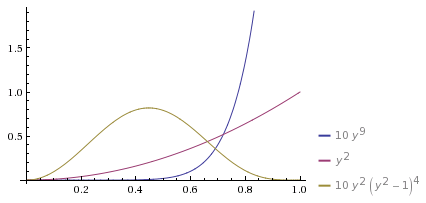
\includegraphics[scale=0.7]{graph1}
		\caption{Graph of $Y_2$, $Y_1'$, and $Y_5'$.}
	\end{figure}
\end{center}

%----------------------------------------------------------------------------------------
%	PROBLEM 3
%----------------------------------------------------------------------------------------

\begin{homeworkProblem}[Exercise\ 3.10.10] % Custom section title
Suppose that $n$ observations are chosen at random from a continuous pdf $f_y(y)$. What is the probability that the last observation recorded will be the smallest number in the entire sample?

\problemAnswer{
\begin{align*}
	P(Y_{min} = Y_n) &= P(Y_n < Y_1, Y_n < Y_2, \dots, Y_n < Y_{n-1})\\
	&=\left(\frac{1}{2}\right)^{n-1}
\end{align*}
}
\end{homeworkProblem}

%----------------------------------------------------------------------------------------
%	PROBLEM 4
%----------------------------------------------------------------------------------------
\begin{homeworkProblem}[Exercise\ 3.11.6]
Let $X$ denote the number on a chip drawn at random from an urn containing three chips, numbered 1, 2, and 3. Let $Y$ be the number of heads that occur when a fair coin is tossed $X$ times.

\begin{homeworkSection}{(a) Find $p_{X,Y}(x,y)$.}
\problemAnswer{
	$p_x(x) = \left(\frac{1}{3}\right)$\\
	$p_{Y \mid X}(x,y) = \dbinom{x}{y}\left(\frac{1}{2}\right)^x, \ y \le x$ \\
	
	So,
	\begin{align*}
		p_{X,Y}(x,y) &= p_{Y \mid X}(y)p_x(x) \\
		&= \dbinom{x}{y}\left(\frac{1}{2}\right)^x\left(\frac{1}{3}\right), \ y \le x
	\end{align*}
}
\begin{homeworkSection}{(b) Find the marginal pdf of $Y$ by summing out the $x$ values.}
\problemAnswer{
	\begin{align*}
		p_Y(0) &= \left(\frac{1}{3}\right)\sum_{x=1}^{3}\dbinom{x}{0}\left(\frac{1}{2}\right)^x \\
		&= \left(\frac{7}{24}\right) \\
		p_Y(1) &= \left(\frac{1}{3}\right)\sum_{x=1}^{3}\dbinom{x}{1}\left(\frac{1}{2}\right)^x \\
		&= \left(\frac{11}{24}\right) \\
		p_Y(2) &= \left(\frac{1}{3}\right)\sum_{x=1}^{3}\dbinom{x}{2}\left(\frac{1}{2}\right)^x \\
		&= \left(\frac{5}{24}\right) \\
		p_Y(3) &= \left(\frac{1}{3}\right)\sum_{x=1}^{3}\dbinom{x}{3}\left(\frac{1}{2}\right)^x \\
		&= \left(\frac{1}{24}\right) \\
	\end{align*}
}
\end{homeworkSection}
\end{homeworkSection}
\end{homeworkProblem}
%----------------------------------------------------------------------------------------
%	PROBLEM 5
%----------------------------------------------------------------------------------------
\begin{homeworkProblem}[Exercise\ 3.11.9]
Let $X$ and $Y$ be independent random variables where $p_x(k) = e^{\lambda(\frac{\lambda^k}{k!})}$ and $p_y(k) = e^{-\mu(\frac{\mu^k}{k!})}$ for $k = 0, 1, ...$. Show that the conditional pdf of $X$ given that $X + Y = n$ is binomial with parameters $n$ and $\frac{\lambda}{\lambda + \mu}$. (Hint: See Question 3.8.1)

\problemAnswer{
	\begin{align*}
		p_{X+Y}(w) &= \sum_{k=0}^w e^{-\lambda} \frac{\lambda^k}{k!} e^{-\mu} \frac{\mu^{w-k}}{(w-k)!} \\
		&= e^{-(\lambda + \mu )} \sum_{k=0}^w \frac{1}{k!(w-k)!} \lambda^{k} \mu^{w-k} \\
		&= e^{-(\lambda + \mu )} \frac{1}{w!} \sum_{k=0}^w \frac{w!}{k!(w-k)!} \lambda^k \mu^{w-k} \\
		&= e^{-(\lambda + \mu )} \frac{(\lambda + \mu)^w}{w!} \\
		\text{conditional pdf is}
		\dots ???
	\end{align*}
}
\end{homeworkProblem}

%----------------------------------------------------------------------------------------
%	PROBLEM 6
%----------------------------------------------------------------------------------------
\begin{homeworkProblem}[Exercise\ 3.11.12]
Given the joint pdf,
\begin{align*}
	f_{X,Y}(x,y) = 2e^{-(x+y)},\quad 0 \le x \le y,\quad  y \ge 0
\end{align*}
\begin{homeworkSection}{(a) $P(Y < 1 \mid X < 1)$}
\problemAnswer{
	\begin{align*}
		f_x(x) &= \int_x^\infty f_{X,Y}(x,y)dy \\
		&= \int_x^\infty 2e^{-(x+y)}dy \\
		&= 2e^{-2x}, \ x > 0 \\
		P(X < 1) &= \int_0^1 2e^{-2x}dx \\
		&= 1-e^{-2} \\
		&= 1-0.135 \\
		&= 0.865 \\\\
		P(X < 1,Y < 1) &= \int_0^1\int_0^x 2e^{-(x+y)}dydx \\
		&= \int_0^1 2e^{-x}[-e^{-y}]_0^x dx \\
		&= \int_0^1 2e^{-x} - 2e^{-2x}dx \\
		&= -2e^{-x} + e^{-2x}\mid_0^1 \\
		&=.4 \\
		\text{Finally,}\\
		P(Y < 1 \mid X < 1) &= \frac{P(X < 1, Y < 1)}{P(X < 1)}\\
		&= \frac{.4}{.87} \\
		&= .46
	\end{align*}
}
\begin{homeworkSection}{(b) $P(Y < 1 \mid X = 1)$}
\problemAnswer{
	$0$. Joint pdf defined as Y always larger than X.
}
\begin{homeworkSection}{(c) $f_{Y\mid x}(y)$}
\problemAnswer{
	\begin{align*}
		f_{Y \mid X}(y) &= \frac{f_{X,Y}(x,y)}{f_x(x)} \\
		&= \frac{2e^{-x+y}}{2e^{-2x}} \\
		&= e^x e^{-y}
	\end{align*}
}
\begin{homeworkSection}{(d) $E(Y \mid x)$}
\problemAnswer{
	\begin{align*}
		E(Y\mid x) &= \int_0^\infty yf_{Y\ mid x}(y)dy \\
		&= e^x \int_0^\infty ye^{-y}dy \\
		&= e^x(-ye^{-y}-e^{-y}) \mid_0^\infty \\
		&= e^x
	\end{align*}
}
\end{homeworkSection}
\end{homeworkSection}
\end{homeworkSection}
\end{homeworkSection}
\end{homeworkProblem}
%----------------------------------------------------------------------------------------
%	PROBLEM 7
%----------------------------------------------------------------------------------------
\begin{homeworkProblem}[Exercise\ 3.11.18]
	Find $P(X < 1 \mid Y = 1\frac{1}{2})$ if $X$ and $Y$ have the joint PDF
	\begin{align*}
		f_{X,Y}(x,y) = xy/2, \quad 0 \le x < y \le 2
	\end{align*}
\problemAnswer{
	\begin{align*}
		f_y(y) &= \int_0^y f_{X,Y}(x,y)dx \\
		&= \int_0^y \frac{xy}{2}dx \\
		&= \frac{x^2y}{4}\mid_0^y \\
		&= \frac{y^3}{4}\\\\
		f_{X \mid y}(x) &= \frac{f_{X,Y}(x,y)}{f_y(y)} \\
		&= \frac{xy/2}{y^3/4} \\
		&= \frac{2x}{y^2}\\
		f_{X \mid \frac{3}{2}}(x) &= \frac{2x}{(3/2)^2} \\
		&= \frac{8}{9}x \\\\
		P(X < ! \mid Y = \frac{3}{2}) &= \int_o^1 f_{X \mid \frac{3}{2}}(x)dx \\
		&= \int_0^1 \frac{8}{9}xdx \\
		&= \frac{4}{9}x^2 \Big|_0^1 \\
		&= \frac{4}{9}
	\end{align*}
}
\end{homeworkProblem}

%----------------------------------------------------------------------------------------
%	PROBLEM 8
%----------------------------------------------------------------------------------------
\begin{homeworkProblem}[Exercise\ 3.11.20]
	Suppose the random variables $X$ and $Y$ are jointly distributed according to the pdf
	\begin{align*}
		f_{X,Y}(x,y) = \frac{6}{7}(x^2+\frac{xy}{2}), \quad 0 \le x \le 1, \quad 0 \le y \le 2
	\end{align*}
\begin{homeworkSection}{(a) $f_{X}(x)$.}
\problemAnswer {
	\begin{align*}
		f_x(x) &= \int_0^2 \frac{6}{7}\left(x^2 + \frac{xy}{2}\right)dy \\
		&= \frac{6}{7}\left(x^2y + \frac{xy^2}{4}\right) \Big|_0^2 \\
		&= \frac{6}{7}(2x^2 + x)
	\end{align*}
}
\begin{homeworkSection}{(b) $P(X > 2Y)$.}
\problemAnswer {
	\begin{align*}
		P(X > 2Y) &= \int_0^1\int_0^{\frac{1}{2}x}\frac{6}{7}\left(x^2 + \frac{xy}{2}\right)dydx \\
		&= \int_0^1\left[\frac{6}{7}\left(x^2y + \frac{xy^2}{4}\right)\right]_0^{\frac{1}{2}x} dx \\
		&= \int_0^1 \frac{6}{7}\left(\frac{9x^3}{16}\right)dx \\
		&= \frac{27}{224}
	\end{align*}
}
\begin{homeworkSection}{(c) $P(Y > 1 \mid X > \frac{1}{2})$}
\problemAnswer {
	\begin{align*}
		P\left(X > \frac{1}{2}, Y > 1\right) &= \int_{\frac{1}{2}}^1\int_1^2 \frac{6}{7}\left(x^2 + \frac{xy}{2}\right)dydx \\
		&= \int_{\frac{1}{2}}^1 \left[\frac{6}{7}\left(x^2y + \frac{xy^2}{4}\right)\right]_1^2 dx \\
		&= \int_\frac{1}{2}^1 \frac{6}{7}\left(x^2 + \frac{3x}{4}\right) \\
		&= \left[\frac{6}{7}\left(\frac{x^3}{3} + \frac{3x^2}{8}\right)\right]_{\frac{1}{2}}^1 \\
		&= \frac{55}{112} \\\\
		\text{Also need to find }
		P\left(X > \frac{1}{2}\right) &= \int_{\frac{1}{2}}^1 \frac{6}{7}(2x^2 + x)dx \\
		&= \frac{23}{38} \\\\
		\text{So, } P(Y > 1 \mid X > \frac{1}{2}) &= \frac{55/112}{23/38} \\
		&= \frac{55}{92}
	\end{align*}
}
\end{homeworkSection}
\end{homeworkSection}
\end{homeworkSection}
\end{homeworkProblem}
\end{document}











